\documentclass{article}
\usepackage{graphicx} % Required for inserting images
\usepackage{makeidx}
\makeindex
\documentclass[12pt]{article}


\title{ \textbf{Sensors Simulator} }
\author{Enrico Cotti Cottini, Mat. 2077993}
\date{Giugno 2024}

\begin{document}

\maketitle

\tableofcontents % Generates the table of contents

\newpage

\section{Introduzione}

Il progetto consiste in un interfaccia grafica in grado di fare interagire l'utente con delle simulazioni di sensori di vario tipo. L'utente può creare, modificare, eliminare e ricercare i sensori inserendone i valori dipendentemente dal tipo di sensore selezionato. I sensori simulati sono sensori di tre diversi tipi: \textbf{temperatura, umidità e qualità dell'aria}. Questi sensori simulano il comportamento metereologico di un certo luogo dati alcuni parametri statistici della località per un certo numero di campionamenti decisi dall'utente. I tre sensori a loro volta implementano una rappresentazione delle condizioni ambientali che misurano, per esempio: 

\begin{itemize}
    \item \textbf{Il Sensore di Temperatura} (da eseguire su n campionamenti) simula la curva di andamento della temperatura (minima massima e attuale) che ha dei cicli notte-giorno dove la notte si misura la temperatura minima e viceversa il giorno la massima. La temperatura viene rappresentata internamente come un oggetto "Temperatura" che contiene i valori di temperatura misurati in Celsius, Fahrenheit e Kelvin gestendo anche i valori di zero assoluto. 
    
    \item \textbf{Il Sensore di Umidità} (da eseguire su n campionamenti) simula la curva di andamento dell'umidità, misurata tramite oggetto interno "Umidità" misurando l'umidità relativa che deve restare entro i valori limite (0\%-100\%). Durante la simulazione il sensore tiene conto dei parametri di probabilità di pioggia e di presenza di pioggia per calcolare l'umidità.
    
    \item\textbf{Il Sensore di Qualità dell'aria}  (da eseguire su n campionamenti) simula la curva di andamento della qualità dell'aria, calcolando lo sviluppo dell'indice della qualità dell'aria basandosi sul comportamento dei valori di pm10 e n02 misurati in microgrammi per metrocubo. Il sensore mostra inoltre i valori limite per contraddistingure in quale fascia di qualità dell'aria ci troviamo, le fasce sono: ottimale, buona, accettabile, mediocre, carente, malsana. 
\end{itemize}

Tutti e tre contengono un valore che indica la deviazione standard del campione che verrà simulato. Questi sensori possono essere salvati e caricati tramite file Json, si può caricare un nuovo file da zero oppure uno già esistente con la possibilita di salvare le modifiche del file caricato precedentemente oppure salvarlo su un altro file specificando il nome.
Aggiungendo un sensore sarà possibile vederlo nella lista dei sensori che presenta tutti i sensori che esistono nella sessione attuale, è possibile riordinarli per ID oppure riordinarli per nome, inoltre possiamo ricercare i sensori in base a ID e nome, possiamo anche modificare il sensore cambiando il tipo oppure i suoi parametri in fine è possibile cancellarlo.
A destra della lista dei sensori è presente la visualizzazione delle informazioni del singolo sensore dove sarà possibile simulare, modificare il sensore oppure pulire i dati raccolti dalla precedente simulazione. 

\section{Descrizione del modello}
\subsection{Modello Logico}
Il modello logico si occupa della rappresentazione degli oggetti sensori e delle condizioni ambientali che misurano. Sono definiti anche il visitor e il constvisitor fondamentali per fare interagire modello logico e grafico.
Partendo dall'alto della gerarchia (Figura 1) con "AbstractSensor" classe virtuale pura che rappresenta il concetto di Sensore. Un sensore ha un Identificatore di tipo unsigned int, un nome come stringa, un dataNum unsigned int che rappresenta il numero di collezioni di dati che devono essere effettuate durante la simulazione. Oltre ai vari metodi getter e setter del caso abbiamo due metodi accept per accettare la visita dei visitor(const e non const) e due metodi virtuali puri. Il metodo "simulate" esegue l'effettiva simulazione riempiendo i contenitori delle condizioni ambientali definiti negli oggetti concreti sulla base di valori iniziali, deviazioni standard e formule diverse per ogni classe concreta con l'obbiettivo di simulare la condizione meteorologica descritta. Il metodo "Clear" pulisce i contenitori che contengono la simulazione. Tramite F1 è possibile visualizzare tutte le scorciatoie da tastiera.

\begin{figure}[h!]
    \centering
    \makebox[\textwidth]{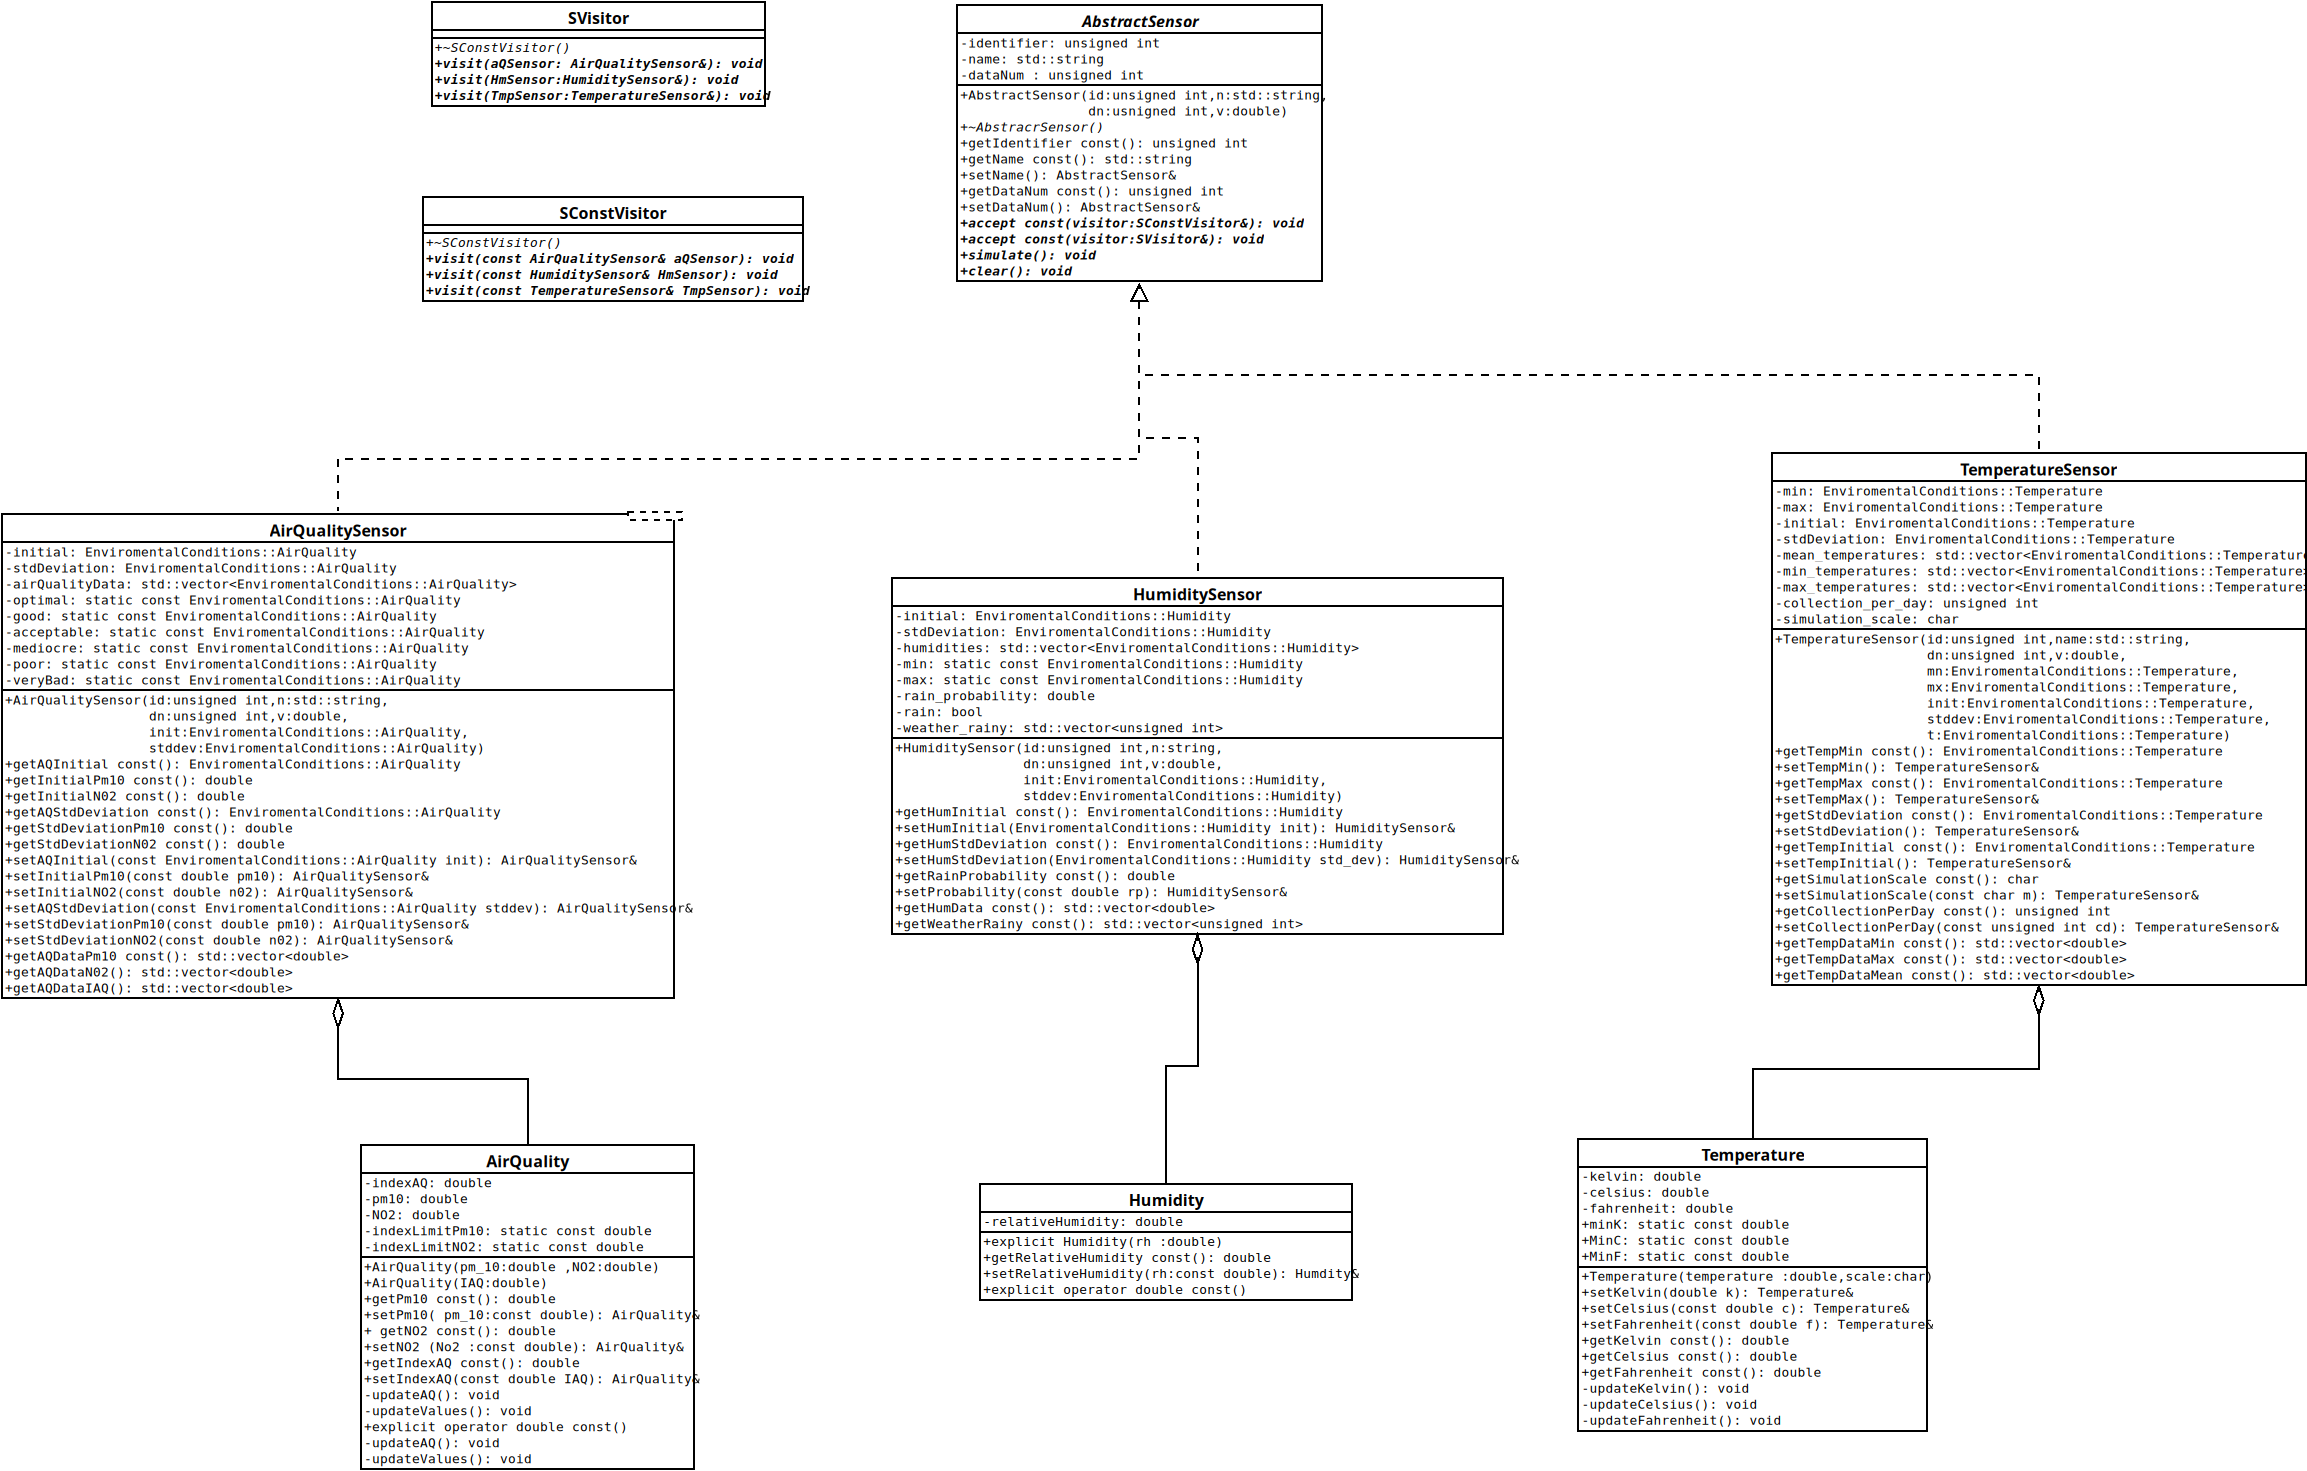
\includegraphics[width=1.3\textwidth]{diagramma-classi.png}}
    \caption{Diagramma UML Modello Logico.}
    \label{fig:example-image}
\end{figure}

\newpage

Di seguito vengono descritte le tre classi concrete:
\begin{itemize}
    \item{\textbf{"TemperatureSensor"} gli argomenti della classe sono: min, max, initial, stdDeviation  che sono di tipo "Temperature", (spiegato nel dettaglio in seguito) questi sono i valori statistici su cui si basa la simulazione. mean\_temperatures, min\_temperatures e max\_temperatures sono i contenitori che contengono i valori di temperatura minima massima e attuale (o media) durante la simulazione. Simulation\_scale indica quale scala di temperatura utilizzare durante la simulazione. Il sensore di temperatura è un caso particolare rispetto agli altri perchè nella sua simulazione tiene conto del ciclo giorno-notte e tramite l'argomento "Collection\_per\_day" possiamo definire quante collezioni di dati fare al giorno. Il ciclo notte-giorno viene simulato tramite una funzione seno e tramite una distribuzione normale i dati sono randomizzati intorno a questa funzione sulla base del valore di deviazione standard.
    \begin{itemize}
        La condizione ambientale \textbf{"Temperature"} è progettata per gestire la temperatura in diverse scale termometriche: Kelvin (K), Celsius (C) e Fahrenheit (F). In particolare updateKelvin(), updateCelsius(), updateFahrenheit() sono utilizzati internamente per aggiornare i valori di temperatura nelle altre scale quando viene impostato un valore in una specifica scala, sono presenti gli zeri assoluti come valori statici.
    \end{itemize}}
    
    \item {\textbf{"HumiditySensor"} gli argomenti della classe sono: initial e stdDeviation che sono di tipo "Humidity", abbiamo inoltre rain probability che indica la probabilità di pioggia e l'attributo booleano rain che indica se piove. oltre al classico contenitore dei dati della simulazione "humidities" abbiamo "weather\_rainy" che contiene in quali iterazioni della collezione dei dati è iniziata o finita la pioggia. I valori max e min membri statici publici rappresentano i limiti 0\%-100\%.
    \begin{itemize}
        La condizione ambientale \textbf{"Humidity"} è progettata per gestire i dati relativi all'umidità. La classe contiene una variabile relativeHumidity di tipo double che rappresenta l'umidità relativa.
    \end{itemize} }
    
    
    \item {\textbf{"AirQualitySensor"}  gli argomenti della classe sono: initial e stdDeviation che sono di tipo "AirQuality". Presenta vari valori statici fia menzionati che rappresentano le soglie limite di qualità dell'aria. Un contenitore per i risultati della simulazione airQualityData. 
    \begin{itemize}
        La condizione ambientale \textbf{"AirQuality"} è progettata per gestire i dati relativi alla qualità dell'aria. Presenta due attributi pm10 e n02, il primo pm10 indica la presenza di particolato sotto i 10\(\mu\text{m}\) misurato in \(\mu \text{g/m}^3\), il secondo indica la presenza di n02 misurata in \(\mu \text{g/m}^3\). Inoltre il terzo attributo "indexAQ" è indice di qualità dell'aria viene gestito ed aggiornato internamente come il tipo Temperatura secondo la seguente formula:
\begin{equation}
    \text{Ipm10} = \left( \frac{\text{pm10}}{\text{indexLimitPm10}} \right) \times 100.0
\end{equation}
\begin{equation}
    \text{INO2} = \left( \frac{\text{NO2}}{\text{indexLimitNO2}} \right) \times 100.0
\end{equation}
\begin{equation}
    \text{indexAQ} = \begin{cases} 
        \text{Ipm10}, & \text{if } \text{Ipm10} \geq \text{INO2} \\
        \text{INO2}, & \text{altrimenti}
    \end{cases}
\end{equation} indexAQ diventa uguale al maggiore tra gli indici calcolati usando indexLimitPm10 indexLimitNO2 che sono valori sempre misurati con la stessa unità di misura che indicano i valori limite massimi oltre al quale la salute potrebbe essere gravemente compromessa, questi valori sono diversi per ogni stato e per l'italia abbiamo \text{indexLimitPm10} = 50.0 \, \mu g/m^3
\quad \text{e} \quad
\text{indexLimitNO2} = 200.0 \, \mu g/m^3

    \end{itemize} }
\end{itemize}

\subsection{Interfaccia Grafica}
L'interfaccia grafica, realizzata tramite il Framework Qt, ha come finestra principale "MainWindow" che è il widget principale della mia applicazione. Qui avviene: creazione, salvataggio e modifica di file json gia nuovi o esistenti, tutti tramite bottoni che trasmettono segnali agli slot publici. Il resto delle operazioni sui sensori come creazione, modifica, delezione, ricerca e ordinamento vengono delegate ai widget figli. Fondamentale è la gestione della memoria che avviene tramite gli atributi "sensor\_list", "repository" e "query" rispettivamente di tipo SensorList(Contenitore da me definito per gestire la memoria dei sensori), JsonRepository(deriva dal supporto nativo di Qt per Json) e SensorList. Questi tre gestiscono la memoria di tutti i sensori della repository json e della query all'attivo. Sui tre argomenti che gestiscono la memoria ho dovuto fare una considerazione; concettualmente sensor\_list, repository e query condividono la stessa memoria perchè se non lo fosse dovrei andare a creare degli oggetti AbstractSensor duplicati inutili, assodato ciò devo stare attento ad usare la stessa memoria assicurandomi di aggiungere le stesse locazioni di memoria nei contenitori. 
Oltre alle funzionalità della "MainWindow" abbiamo dei widget figli che hanno a loro volta altre funzionalità.
"EditWidget" il widget per creazione di nuovi sensori o modifica di quelli esistenti, queste due operazioni avvengono dinamicamente. Per creare un nuovo sensore bisogna cliccare il bottone "create\_sensor" presente nella toolbar oppure tramite la scorciatoia da tastiera (CTRL + N), apparirà una nuova finestra con uno dei campi da compilare, in particolare un menù a tendina ci permetterà di selezionare il tipo di sensore che vogliamo creare. Se vogliamo modificare un sensore pre-esistente il programma tramite due Visitor capisce il tipo dinamico del sensore e gli assegna il corrispettivo editor. "SensorListWidget" è il widget che gestisce la visualizzazione della lista dei sensori attivi, ogni sensore viene mostrato, tramite un renderer che fa utilizzo di un visitor, con il suo tipo, il nome, l'ID e tre bottoni per visualizzare tutte le informazioni, modificare e cancellare il sensore. Per la modifica viene chiamato un metodo della "MainWindow" che a sua volta crea un "EditWidget" che fa il resto del lavoro, la delezione del sensore viene gestita internamente a "SensorListWidget", mentre la visualizzazione di tutte le informazioni del sensore viene delegata a sua volta a "SensorWidget". Quest'ultimo è membro di "MainWindow" e rappresenta la schermata principale in cui avviene la simulazione del sensore, questo lo fa tramite un renderer e un simulator. Il renderer renderizza l'intera pagina del sensore comprese informazioni e un grafico, implementato tramite QtCharts per raccogliere e mostrare i dati ricavati dalla simulazione. Il simulatore raccoglie i dati generati dalla simulazione dei sensori e li inserisce nel grafico per mostrarli all'utente, entrambi questi due oggetti fanno utilizzo di visitor per gestire il tipo dinamico del sensore. In fine abbiamo il "SearchWidget" che raccoglie il testo della query che vogliamo effetuare e richiama "MainWindow" che cerca nella propria memoria se trova dei sensori che soddisfano la query.

\section{Descrizione dell'utilizzo non banale del polimorfismo}

Ho utilizzato ampiamente il design pattern del visitor che mi è stato di ausilio per la progettazione di renderizzatori, editor e simulatori:
\begin{itemize}
    \item il \textbf{"SensorRenderer"} è il renderizzatore che mostra le varie informazioni del sensore insieme al grafico della simulazione, facendosi aiutare da un ConstVisitor "Full" che appunto visita il sensore per capire la tipologia di questo e riempie i sui campi dipendentemente da ciò.
    \item \textbf{"GraphSimulator"} è colui che effettua la chiamata della simulate() del sensore e ne raccoglie i dati per inserirli nel grafico. Un Visitor "SimulationVisitor" visita il sensore e riceve i dati delle simulazioni che vengono trattati diversamente in base al tipo del sensore. Nel caso del sensore di temperatura se il numero di campionamenti è abbastanza contenuto viene utilizzato un grafo con QStackedBarSeries che permette una visualizzazione dei massimi e minimi come intervalli continui. In tutti gli altri casi viene usato QLineSeries.
    \item \textbf{"ListRenderer"} è il renderizzatore della lista dei sensori disponibili e ha una gerarchia simile al "SensorRenderer". Il renderer si può differenziare in più strategie (nel mio caso solo una) utilizzando un ConstVisitor che decide il tipo dinamico e mostra a schermo una piccola iconcina del tipo del sensore e i dati di ID e nome.
    \item \textbf{"SensorEditor"} è la gerarchia degli editor di sensori. Esiste una classe astratta AbstractSensorEditor che funge da astrazione degli editor per ogni tipologia di sensore. Inoltre tramite due visitor l'"EditWidget" può chiamare l'editor adatto per quel sensore.
\end{itemize}

\section{Persistenza dei dati}

Per la persistenza dei dati viene utilizzato il formato JSON e in un solo file vengono salvati tutti i sensori di una sessione. La gestione del tipo di sensore viene fatta aggiungendo un attributo type.
Per provare ad avere i sensori con i dati statistici più realistici ho creato un piccolo API in python e bash che preleva i dati da "https://openweathermap.org/" ogni 10 minuti e ne fa un'analisi statistica riportando i sensori in JSON, pronti per essere utilizzati dal programma, per 20 città italiane diverse. Questo non credo sia materiale di giudizio del corso però ho pensato di farlo per avere dei sensori basati su dati reali. Detto Questo i JSON presenti per ogni città contengono tutti e tre i sensori basati sui dati che vanno dal 30/05/2024 al 16/06/2024. Le 20 città in questione (con relative coordinate) sono:
\begin{itemize}
\item Roma: 41.8947, 12.4839
\item Milano: 45.4643, 9.1895
\item Napoli: 40.8333, 14.25
\item Torino: 45.1333, 7.3667
\item Palermo: 37.8167, 13.5833
\item Genova: 44.5, 9.0667
\item Bologna: 44.4667, 11.4333
\item Firenze: 43.7667, 11.25
\item Bari: 41.1177, 16.8512
\item Catania: 37.5021, 15.0872
\item Venezia: 45.4386, 12.3267
\item Verona: 45.4167, 11.0333
\item Messina: 38.1933, 15.5497
\item Padova: 45.4152, 11.8818
\item Trieste: 45.6486, 13.78
\item Taranto: 40.6167, 17.25
\item Brescia: 45.6333, 10.3
\item Parma: 44.8027, 10.329
\item Prato: 43.8843, 11.0909
\item Modena: 44.5, 10.9
\end{itemize}

\section{Funzionalità implementate}

Le funzionalità implementate sono:
\begin{itemize}
    \item Gestione di tre tipi di Sensori di Condizioni Ambientali, creazione, delezione e modifica;
    \item Creazione e salvataggio di File Json di sensori;
    \item Visualizzazione dei sensori sotto forma di lista con cui l'utente può interagire;
    \item Ordinamento della lista dei sensori in base a ID o Nome;
    \item Ricerca dei Sensori tramite search bar; 
    \item Simulazione di sensori;
    \item Visualizzazione tramite Grafico di QtChart dei dati simulati;
    \item Controllo degli ID, diversi sensori non possono avere ID uguali;
    \item Status bar; 
    \item Le finestre e gli widget adattano la loro dimensione;  
    \item ToolBar;
    \item Scrociatoia da testiera: Create: Ctrl + Shift + C
Open: Ctrl + O
Save: Ctrl + S
Save As: Ctrl + Shift + S
Create Sensor: Ctrl + N
Help: F1;
    \item Gli Widget Lista e Grafico possono essere sovrapposti scorrendo il divisore.
\end{itemize}

\section{Rendicontazione delle ore}

\begin{table}[h!]
\centering
\begin{tabular}{|c|c|c|}
\hline
\textbf{Attività} & \textbf{Ore Previste} & \textbf{Ore Effettive} \\
\hline
Studio e progettazione & 10 & 10 \\
\hline
Sviluppo del codice del modello & 20 & 20 \\
\hline
Studio del framework Qt & 10 & 20 \\
\hline
Sviluppo del codice della GUI & 15 & 25 \\
\hline
Test e debug & 10 & 20 \\
\hline
Stesura della relazione & 5 & 5 \\
\hline
\textbf{totale} & 70 & 100 \\
\hline
\end{tabular}
\end{table}

Le mie considerazioni iniziali sui tempi sono state abbondanti rispetto al monte di 50 ore, questo perchè avevo gia previsto di prendere un po' più con calma il progetto dato che è il primo lavoro serio da me svolto così da poter imparare bene anche i mezzi e i metodi per lo sviluppo del software. In più parallelamente a questo ho provato a sviluppare un progetto con lo stesso modello logico ma l'interfaccia grafica tramite QtDesigner messo a disposizione di QtCreator, dopo diverse ore di sviluppo ho deciso di prediligere l'approccio senza l'utilizzo di QtDesigner.

\section{Considerazioni finali}

Durante lo sviluppo di questo progetto ho preso familiarità con Qt, c++, design patterns oltre a altri mezzi per lo sviluppo software tra cui gli IDE VisualStudioCode e CLion(attualmente il mio preferito), il VCS git e la piattaforma github, GDB(setuppato su CLion) per effettuare il debugging, che è stato una manna dal cielo per fixare i segmentation fault, Valgrind mezzo assolutamente stupendo che mi ha permesso di fixare errori e Memory Leaks. Ho notato che Wayland il gestore delle finestre standard  di Ubuntu va in conflitto con qt creando alcuni memory leak e altri errori sulla visualizzazione delle finestre.

\end{document}
